\documentclass[../main/main.tex]{subfiles}

\begin{document}

\chapter{Introduction and basic definitions}

\begin{chapquote}{Lucretius}
    "Non erit, et lux solis flare nos de tenebris et rerum scientia".
\end{chapquote}

% \begin{chapquote}{William of Ockham}
%     The simplest explanation is most likely the right one.
% \end{chapquote}

\newdate{date}{02}{03}{2023}

\marginpar{ \textbf{Lecture 1.} \\  \displaydate{date}. \\ Compiled:  \today.}

Physics has always been the combination of experiments and theory. Since Galileo, the observation had always been the starting point to apply the scientific method, followed by hypothesis, deductions and experimental controls.  
What makes physics an \emph{exact science} is the fact that it is based on mathematical models and principles that are consistently observed in the natural world. These mathematical models allow physicists to make precise predictions about the behavior of physical systems and the results of experiments, which can then be tested through further observations and experiments.
In the history of physics many times had happened that theory had predicted reality - think of the Higgs boson - and from this we had learnt that we have a so good comprehension of reality that we are often capable to predict and describe its most inner aspects.
On the other hand, biology has not had the same luck: compared to physics, in which, again, both theory and experiments allow us to gain knowledge about reality, there is not a rigorous mathematical theory behind biology.
There are not always rigorous models able to describe biology. The study of biology is essentially the study of complexity.
Even if \emph{complexity} it's further the goals of this course, we can think of that as the mathematician Peter Dodds would describe it: \emph{"There's no love in a carbon atom, No hurricane in a water molecule, No financial collapse in a dollar bill."} \cite{complexity}.
Biological Physics is basically the study of this complexity with goal the understanding of the physics behind this complexity, behind biology. 
Contrary to a basic course in physics, in which we could start from the laws of Newton of motion, here there are no Newton's laws in biological physics. By making the assumption that the motion is in absence of friction and that the objects move with constant velocity horizontally and accelerating vertically \emph{"If then the balls of lead, of iron, of stone do not observe that supposed proportion, its damage, we will say that we are not talking about them."} as Evangelista Torricelli would say\footnote{Se poi le palle di piombo, di ferro, di pietra non osservano qella supposta proporzione, suo danno, noi diremo che non parliamo di esse. \cite{E-Torricelli}}.

The key problem is that every biological particle moves in a dissipative medium, which cannot be neglected: \textbf{water}.
This actually impose the need to work in a specific framework which is not the traditional one, but it's the stochastic one. We will then deal with stochastic equations.
It is important to underline that, since we are working in water, we will work at low \textbf{Reynolds-number} so in a regime in which $\vec{F}\propto \vec{v}$ and not $\vec{a}$. Also the $\vec{\nabla}$ operator will be use, expecially in everything concerning fluidodynamics and we will pay attention to tha \href{https://en.wikipedia.org/wiki/Del_in_cylindrical_and_spherical_coordinates#Del_formula}{many representations} this operator shows.
Moreover, it is relavant to rememeber that the usual time reversal property is no longer possible as we cannot keep track of an Avogadro's number ($N_A$) of particles. 
What we wish to show, thanks to statistical mechanics, the \emph{Langevin equantion} and the \emph{Fokker-Planck equations}, is that nature tends to use the same strategies and ideas over and over again. Basically, we will deal with many applications, in order to emphasize that biological physics is an applied subject rather than only a theoretical one. 
We will start then by considering a single particle moving in water. Then we will exdend this argument to many particles diffusing in water and we will give some possible applications.

\section{Elements of thermodynamics: statistical mechanics}
Since it is not possible to study $N_A\approx10^{23}$ particles statistical mechanics is the practical solution to use in order to connect biology and physics.\\
In thermodynamics we have two representations: \textbf{entropic} and \textbf{energetic} representation.
% \subsection{Entropy representation}
Equilibrium thermodynamics in terms of entropy representation express the entropy $S$ as a function of linearly additive (extensive) variables: the internal energy, the volume and the number of particles: $$S=S(U, V, N).$$
% \subsection{Energy representation}
Instead, in terms of energy representation, it is possible to invert the the above equation and express the internal energy $U$ as a function of $U=U(S, V, N)$. This equation is less fundamental than the previous one, but it is more used. From this we can generate the \emph{free energies} which are fundamental statical quantities that are equivalent to internal energy with the difference that, using \emph{Legendre transformations}, an extensive parameter is replaced with an intensive one.
For example, by replacing the entropy $S$ with the temperature $T$ we get the Helmholtz free energy $F=F(T,V,N)$ or by replacing also the volume $V$ with the pressure $P$ and we get the Gibbs free energy $G=G(T,P,N)$ and so on.
These frameworks will be useful to understand ions pumps, thanks to which neurons are able to communicate and work properly in a non-equilibrium environment, or molecular motors, proteins folding, two-states systems (like the folding and unfolding process of RNA using \emph{optical tweezers}), how polymers behave, how they interact and transform, what are their shapes and properties and many many other cases.  

To investigate the link with biology let's consider this example:
\begin{figure}[ht!]
    \centering
    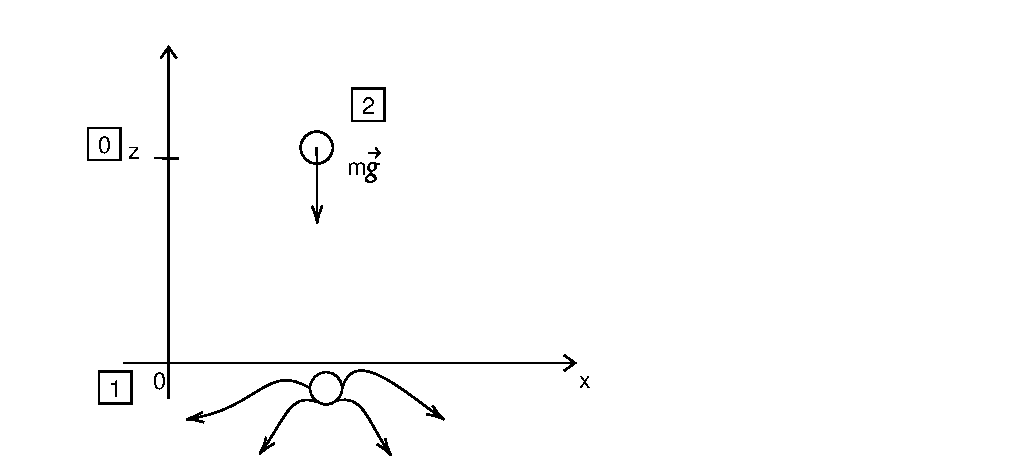
\includegraphics[width=0.6\textwidth]{../frontespizio/tikz/0_lesson/00_1.pdf}
    % \label{fig:9_1}
    \caption{Heat and conservation of energy}
\end{figure}
A particle starts at rest at height $z$ is subjected to an external field force $\vec{g}$ pointing downward. The particle has total internal energy $U = \frac{1}{2}m\vec{v}^2(t)+mgz(t)$. By neglecting the action of air
\begin{equation*}
    \begin{split}
        \frac{d}{dt}U(t) & =\underbrace{\frac{1}{\cancel{2}}m\cancel{2}\vec{v}\cdot\frac{d}{dt}\vec{v}}_{\frac{d\vec{v}}{dt}=(0,0,-g)=\vec{a}}+mg\underbrace{v_z(t)}_{\vec{v}=(0,0,v_z(t))}\\
        & = \underbrace{-mgv_z(t)}_{>0}+\underbrace{mgv_z(t)}_{<0}\stackrel{!}{=} 0
    \end{split}
\end{equation*}
This proves that the internal total energy is conserved, as we know from this simple physics problem.
We can consider then $\Delta U = U_1-U_0 = Q$ which represents the total heat absorbed by the system.\\
Supposing that the ground is made of mud, then energy is transformed to the mud as heat $Q$, so there is a dissipation of energy. If we consider also step \framebox[0.5cm][c]{2} we can write, since we are considering a cyclic transformation
\begin{equation}
    \begin{split}
        \Delta U &= U_2-U_0 = \underbrace{U_2-U_1}_{W}+\underbrace{U_1-U_0}_{Q}\\
        &=W+Q
    \end{split}
\end{equation}
where $W$ is the work absorbed by the system. In the case in which there is no mud $\Delta U = 0$, but since we generally do not deal with cyclic transformations the above $\Delta U = W+Q$ represents the conservation of the total energy, also known as the $1^{st}$ law of thermodynamics. We underline the fact that the $\Delta$ is present due to the fact that $U$ is a function of state, while $W$ and $Q$ are not. 

The link to biology with this example can be found by considering the case in which the mud is warmed up when the particle hit it: in this case there is a dissipation of energy and the particle is not able to come back to the starting point, due to the fact that we have to take into account the $2^{nd}$ law of thermodynamics too. In the Helmholtz framework, the Helmholtz free energy is given by $F=F(T, V, N) = U-TS$ where entropy is used to estimate the fraction of \emph{low quality energy}. \\
The key idea is that the entropic term depicts the disorder of the system and it is linked directly to the energy that the system can no longer use. The amount of \emph{good quality energy} the system loses depends on the temperature: the higher the temperature the more the \emph{good energy} is lost.
For biology this is of utmost importance because, since there is no molecular machine that works a $0$ temperature, nature uses disorder to produce work, by further continuously find a trade-off between temperature level and quantity of disorder. In this particular range of temperatures - $T=T_r$ is the temperatureof the larger system, called \emph{thermal reservoir} - biology works and it is able to commute outside good energy into low quality one and also to take advantage of the disorder-entropic component in someway.
Since every biological system is not a closed system but it is always in touch with a greater system a \emph{reservoir}, it is possible to have $\Delta S <0$. 
For an open system we can the restate the second law of thermodynamics as 
\begin{equation}
    \frac{\Delta U}{T} \leq \Delta S \implies \Delta F \leq 0
\end{equation}    
to underline the possibility of the system to control and reuse entropy, in order to improve the order of the system, as far as the good quality energy, coming from outside, is used and reduced by a proper amount ($2^{nd}$ law) and converted into low quality ($1^{st}$ law) which is ejected in the surrounding. The free energy, so the energy available to perform work, decreases if the open system realizes a spontaneous process.
\end{document}
